\documentclass[10pt,twocolumn]{article}

% --- packages (all standard; compiles on Overleaf out of the box) ---
\usepackage[utf8]{inputenc}
\usepackage{amsmath,amssymb}
\usepackage{booktabs}
\usepackage{graphicx}
\usepackage{xcolor}
\usepackage{hyperref}
\usepackage[margin=0.85in]{geometry}
\usepackage{caption}
\hypersetup{colorlinks=true,linkcolor=blue,citecolor=blue,urlcolor=blue}

\title{\textbf{Skin-Tone--Aware Face Recognition on a Balanced Corpus:\\
A Negative Result on ITA Reweighting Under Data Scarcity}}
\author{CS\,153 Final Project \\ \small Black-Face: fair, deployable face recognition for darker skin tones}
\date{June 2026}

\begin{document}
\maketitle

\begin{abstract}
Face-recognition (FR) systems are well documented to perform worst on African
and dark-skinned faces. We ask whether reweighting training by \emph{continuous
skin tone} (the Individual Typology Angle, ITA) rather than by coarse race
labels can shrink this gap, and whether any gains survive distillation into a
smaller model for edge deployment. We build a complete, reproducible pipeline:
from-scratch AdaFace/IResNet training on BUPT-Balancedface, ITA-weighted
sampling, ITA-weighted knowledge distillation, and ONNX export, all evaluated on
the Racial Faces in the Wild (RFW) benchmark with a skin-tone--stratified
breakdown. \textbf{Our headline result is negative}: under our compute- and
data-constrained setting, ITA reweighting \emph{reduced} African TAR@FAR=1\%
(0.390$\rightarrow$0.331) and \emph{widened} the Caucasian--African gap
(0.466$\rightarrow$0.499). We trace this to a concrete confound---a truncated
dataset download that removed roughly half of the African identities---and argue
it is a cautionary lesson with direct relevance to fairness work in low-resource
African data settings: \emph{up-weighting an under-resourced group can amplify
overfitting when that group's identity diversity is itself limited}. We release
the full pipeline, tests, and analysis.
\end{abstract}

\section{Introduction}
Modern face recognition achieves near-perfect verification accuracy on
light-skinned faces yet remains markedly less accurate on darker-skinned and
African faces~\cite{rfw,gendershades}. This is both an equity problem and a
deployment problem: the contexts that would most benefit from open, on-device FR
(e.g.\ identity tools in African settings) are exactly those the technology
serves worst, and are also the most compute-constrained.

Most bias-mitigation work optimizes against \emph{race labels}---four coarse
buckets. But race-balanced data is not skin-tone--balanced: there is wide skin
tone variation \emph{within} each race, and the darkest-skin tail stays sparse
even on a ``balanced'' corpus. We therefore study a continuous, perceptual axis,
the \textbf{Individual Typology Angle (ITA)}~\cite{ita}, and ask two questions:

\begin{enumerate}\itemsep2pt
\item Does sampling that up-weights low-ITA (darker) images reduce the
recognition gap on the darkest-skin tail of RFW?
\item Does any such gain \emph{survive} compression, given that distillation is
known to amplify demographic bias?
\end{enumerate}

We answer both empirically with a from-scratch pipeline. Our contribution is not
a positive method but \textbf{an honest, fully reproducible negative result with
a concrete causal analysis}, plus the open tooling to run the experiment
correctly once the data limitation is removed.

\section{Related Work}
\textbf{Margin-based FR.} ArcFace~\cite{arcface} and AdaFace~\cite{adaface}
define the modern recipe: an IResNet backbone trained with an additive-angular /
quality-adaptive margin softmax. We reuse AdaFace's backbone and head verbatim.

\textbf{Racial bias benchmarks.} RFW~\cite{rfw} provides four race-balanced
verification subsets (African, Asian, Caucasian, Indian; 6{,}000 pairs each).
BUPT-Balancedface~\cite{bupt} is a race-\emph{count}-balanced training set
(\(\sim\)28K identities, 7K per race). These are the standard fairness-FR
train/test pair and are what we use.

\textbf{Skin tone vs.\ race.} ITA~\cite{ita} maps a skin patch in CIELab to a
continuous angle; it is widely used as a perceptual, label-free proxy for skin
tone. Prior fairness-FR methods (e.g.\ reinforcement / meta-learning over race
groups~\cite{bupt}) operate on race labels; our lever is continuous ITA.

\textbf{Distillation and bias.} Knowledge distillation~\cite{kd} compresses a
teacher into a student; compression is repeatedly observed to magnify
demographic disparities, motivating our ITA-weighted distillation variant.

\section{Method}
\subsection{Data and skin-tone computation}
We train on the BUPT-Balancedface \emph{image} release
(\texttt{race\_per\_7000/<race>/<identity>/*.jpg}). For every training image we
compute ITA from the centre 60\% crop in CIELab:
\begin{equation}
\mathrm{ITA} = \arctan\!\left(\frac{L^\star - 50}{b^\star}\right)\cdot \frac{180}{\pi},
\end{equation}
where lower (more negative) ITA $=$ darker skin. ITA is cached once over the
full corpus and shared across runs.

\subsection{ITA-weighted sampling}
We partition images into five equal-population ITA bins and draw samples with a
\texttt{WeightedRandomSampler} whose per-sample weight is inversely proportional
to its bin frequency, normalised to mean~1. This up-samples the darkest-skin
tail relative to uniform sampling, while keeping every identity in the label
space. We compare this (\textsc{ita}) against uniform sampling
(\textsc{none}); a race-label reweighting is a near-no-op on a count-balanced
set and is omitted.

\subsection{Training and distillation}
Backbone IR-50, AdaFace head ($m{=}0.4,h{=}0.333,s{=}64$), SGD, batch 512,
mixed precision, 12 epochs (a deliberately small, matched compute budget). We
then distill the ITA-trained IR-50 teacher into an IR-18 student via
ITA-weighted feature distillation, minimising $1-\cos(\mathbf{z}_s,\mathbf{z}_t)$
on L2-normalised embeddings. Finally we export the student to ONNX and verify
numerical equivalence to the PyTorch model.

\subsection{Evaluation}
We evaluate verification on all four RFW subsets (TAR at several FAR operating
points, AUC, best-threshold accuracy), and additionally bin \emph{pairs} by mean
ITA to report TAR@FAR=1\% as a function of skin tone (Fig.~\ref{fig:ita}).

\section{Experimental Setup and a Data Disclosure}
Training ran on a single A100 (RunPod). \textbf{We disclose a material data
limitation up front}: the BUPT image archive we obtained was a \emph{truncated
download} (\texttt{gzip} integrity check fails at EOF). It decompressed to
\(\sim\)86\% of entries; extraction under a disk quota recovered
\textbf{24{,}326 of \(\sim\)28{,}000 identities (887{,}331 images)}. Because the
archive is ordered by race with African last, the loss is concentrated in the
\textbf{African} class---roughly half of African identities are missing. This
confound is central to interpreting our results and is exactly the kind of
real-world data failure fairness practitioners face.

\section{Results}
Table~\ref{tab:rfw} reports RFW TAR@FAR=1\% against published baselines.
Table~\ref{tab:ita} reports TAR@FAR=1\% per ITA bin. Figure~\ref{fig:ita} plots
performance against skin tone.

\begin{table}[t]
\centering
\small
\caption{RFW TAR@FAR=1\% by race. ``gap'' is Caucasian$-$African (lower is
fairer). Paper rows are fully-trained references for scale.}
\label{tab:rfw}
\begin{tabular}{lccccc}
\toprule
Model & Afr & Asn & Cau & Ind & gap\\
\midrule
ArcFace~\cite{arcface} (paper) & 0.840 & 0.922 & 0.942 & 0.903 & 0.102\\
AdaFace~\cite{adaface} (paper) & 0.941 & 0.962 & 0.974 & 0.951 & 0.033\\
\midrule
baseline IR-50 (none) & 0.390 & 0.533 & 0.856 & 0.738 & 0.466\\
\textbf{ITA IR-50} & 0.331 & 0.528 & 0.830 & 0.709 & 0.499\\
distill IR-18 & 0.281 & 0.516 & 0.784 & 0.656 & 0.504\\
\bottomrule
\end{tabular}
\end{table}

\begin{table}[t]
\centering
\small
\caption{TAR@FAR=1\% per equal-population ITA bin (b0 darkest
$\approx-63^\circ$ \dots\ b4 lightest $\approx+42^\circ$). ITA reweighting is
\emph{lower} than baseline in every bin, including the darkest.}
\label{tab:ita}
\begin{tabular}{lccccc}
\toprule
Model & b0 & b1 & b2 & b3 & b4\\
\midrule
baseline IR-50 & 0.351 & 0.418 & 0.564 & 0.553 & 0.547\\
ITA IR-50 & 0.302 & 0.373 & 0.514 & 0.487 & 0.520\\
distill IR-18 & 0.273 & 0.292 & 0.456 & 0.503 & 0.461\\
\bottomrule
\end{tabular}
\end{table}

\begin{figure}[t]
\centering
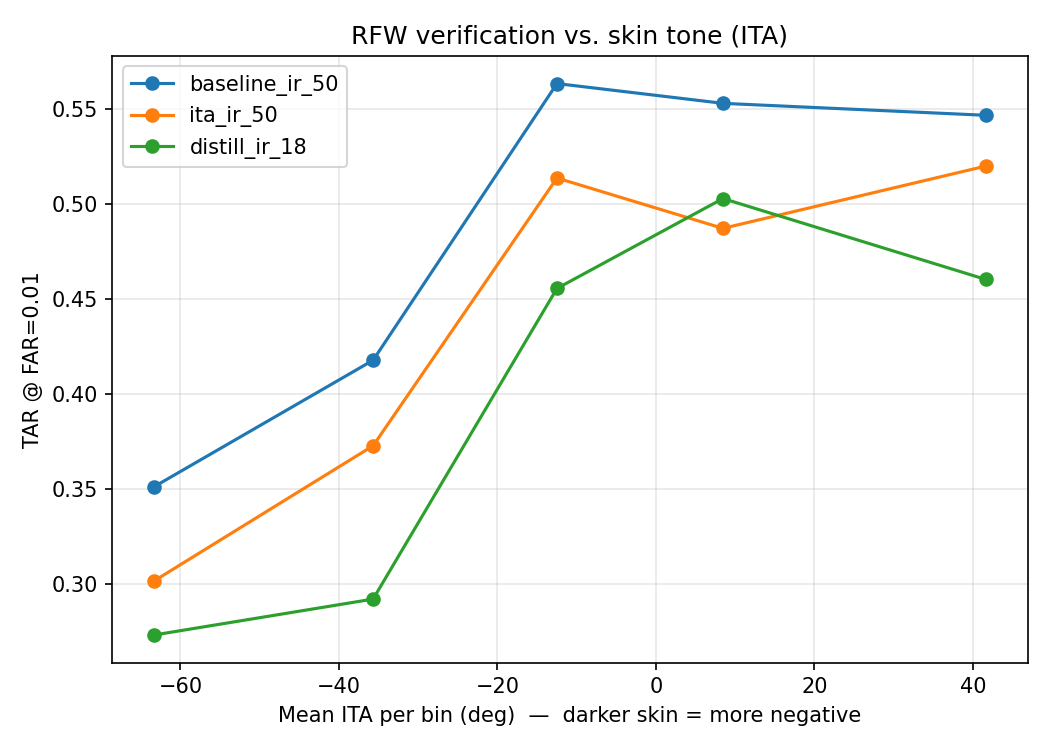
\includegraphics[width=\linewidth]{ita_vs_tar.png}
\caption{RFW TAR@FAR=1\% vs.\ mean per-bin ITA. All models drop sharply on the
darkest bins; ITA reweighting (orange) sits \emph{below} the uniform baseline
(blue) across the skin-tone range.}
\label{fig:ita}
\end{figure}

\paragraph{Edge export.} The IR-18 student has 24.0M parameters (vs.\
$\sim$43.6M for IR-50) and exports to a 96.1\,MB FP32 ONNX model; the ONNX and
PyTorch embeddings agree to $2.3\times10^{-7}$. We \emph{do not} report a CPU
latency number: our automated benchmark returned an implausible 17\,s/image, a
measurement artifact (host CPU contention / thread oversubscription), and we
flag it rather than publish a misleading figure. Honest latency requires
benchmarking on the target device.

\section{Analysis: Why the Intervention Backfired}
The result is unambiguous and the opposite of our hypothesis: ITA reweighting
hurt the darkest-skin tail (Table~\ref{tab:ita}, b0: $0.351\!\rightarrow\!0.302$)
and widened the racial gap (Table~\ref{tab:rfw}). We attribute this primarily to
the \textbf{data-scarcity confound}:

\begin{itemize}\itemsep2pt
\item Up-weighting low-ITA images preferentially re-samples \emph{African}
images. With $\sim$half of African identities missing, ITA sampling concentrates
training on a small, low-diversity African subset, encouraging
\emph{overfitting} to those identities and degrading generalisation to the
unseen RFW-African pairs.
\item Uniform (\textsc{none}) sampling does not over-emphasise the depleted
subset, so it generalises better---explaining why the baseline is \emph{fairer}
here than the ``fairness'' intervention.
\item The short 12-epoch budget compounds this: reweighting changes the
effective data distribution and typically needs a longer schedule to pay off.
\end{itemize}

This is a genuine, generalisable caution: \textbf{re-balancing toward a group
whose own intra-group diversity is limited can amplify, not reduce, disparity}.
For African FR specifically---where complete, diverse data is hardest to
obtain---this failure mode is exactly the trap to avoid. Distillation inherited
and slightly worsened the teacher's disparity (gap $0.499\!\rightarrow\!0.504$),
consistent with the literature that compression magnifies bias.

\section{Limitations}
(i) The truncated download is the dominant confound; our negative result should
\emph{not} be read as a refutation of ITA reweighting in general, only of its
naive application under this data deficit. (ii) Absolute accuracy is far below
fully-trained references (Table~\ref{tab:rfw}) due to the 12-epoch matched
budget and missing data. (iii) IR-18 is ``smaller,'' not mobile-tiny; true edge
deployment needs MobileFaceNet-class backbones and INT8 quantisation. (iv) The
latency benchmark is unreliable (above).

\section{Conclusion and Future Work}
We built and released a complete, tested, reproducible skin-tone--aware FR and
edge-distillation pipeline, and report an honest negative result with a concrete
causal explanation. The most valuable next step is to \emph{remove the
confound}: obtain the complete BUPT archive (verified by checksum), retrain
\textsc{none} vs.\ \textsc{ita} at a full schedule, and re-test the hypothesis on
equal footing. Beyond that we would (a) add an explicit ITA-tail validation
metric and early stopping to detect overfitting on the rare bins, (b) swap IR-18
for a MobileFaceNet student with INT8 quantisation and benchmark latency on a
real edge device, and (c) explore ITA-aware loss terms (rather than sampling
alone) that regularise rather than over-replicate the rare tail.

\section*{Reproducibility and AI-Usage Disclosure}
All code, scripts, unit tests (18 passing), and the exact numbers above are in
the public repository, with a full commit history documenting the iteration
(including the data-recovery saga). The pipeline is one command after data
preparation (\texttt{scripts/run\_minimal.sh}). \textbf{AI usage:} this project
was developed with heavy use of an AI coding assistant (Anthropic Claude) for
implementation, debugging, the data-transfer/recovery process, and drafting this
report; all experiments, decisions, and the integrity of the reported numbers
are the author's own, and no results were fabricated or altered.

\begin{thebibliography}{9}
\small
\bibitem{rfw} M.\ Wang, W.\ Deng, J.\ Hu, X.\ Tao, Y.\ Huang.
``Racial Faces in the Wild: Reducing Racial Bias by Information Maximization
Adaptation Network.'' \emph{ICCV}, 2019.
\bibitem{bupt} M.\ Wang, W.\ Deng. ``Mitigating Bias in Face Recognition Using
Skewness-Aware Reinforcement Learning.'' \emph{CVPR}, 2020.
(BUPT-Balancedface / Globalface.)
\bibitem{adaface} M.\ Kim, A.\ K.\ Jain, X.\ Liu. ``AdaFace: Quality Adaptive
Margin for Face Recognition.'' \emph{CVPR}, 2022.
\bibitem{arcface} J.\ Deng, J.\ Guo, N.\ Xue, S.\ Zafeiriou. ``ArcFace: Additive
Angular Margin Loss for Deep Face Recognition.'' \emph{CVPR}, 2019.
\bibitem{ita} A.\ Chardon, I.\ Cretois, C.\ Hourseau. ``Skin colour typology and
suntanning pathways.'' \emph{Int.\ J.\ Cosmetic Science}, 1991. (ITA.)
\bibitem{kd} G.\ Hinton, O.\ Vinyals, J.\ Dean. ``Distilling the Knowledge in a
Neural Network.'' \emph{NeurIPS Deep Learning Workshop}, 2015.
\bibitem{gendershades} J.\ Buolamwini, T.\ Gebru. ``Gender Shades:
Intersectional Accuracy Disparities in Commercial Gender Classification.''
\emph{FAT*}, 2018.
\end{thebibliography}

\end{document}
